
\documentclass{article}

% Lenguaje y Fuente
\usepackage[spanish]{babel}
\usepackage[utf8x]{inputenc}
\usepackage[T1]{fontenc}
\usepackage[top=1in, bottom=1.25in, left=1.1 in, right=1.1 in]{geometry}
\usepackage{graphicx}
\usepackage{ragged2e}

% Portada

\title{\textbf{Reporte de la Actividad 2}\\ Introducción a Python y Jupyter Lab}
\author{Luis Fernando Duarte Gonzalí \\ Universidad de Sonora \\ Física Computacional}
\date{Enero del 2019}
\begin{document}
\maketitle

% Contenido del Reporte

\section{Introducción}
\justify
En el siguiente trabajo se muestra una actividad realizada para conocer el entorno de \textsc{Jupyter Lab} y el uso de un lenguaje de programación \textit{\textsc{Python}} en el cual se muestran los resultados del análisis de datos registrados por el servicio meteorológico nacional en Nogales, Sonora. Los datos registrados datan del 24 al 31 de Enero del presente año.

El análisis de datos se hizo a través de \textbf{python}, se realizaron las gráficas las ráfagas, la velocidad y la dirección del viento registrado en esos días, además de la radiación solar y otros parámetros.

\section{Estación Meteorológica Automática}
\justify
Es un conjunto de dispositivos eléctricos y mecánicos que realizan mediciones de las variables meteorológicas de forma automática (sobre todo en forma numérica) (Referencia OMM 182.).

Una Estación Meteorológica Automática, está conformada por un grupo de  sensores  que  registran  y   transmiten  información  meteorológica de forma automática de los  sitios  donde están estratégicamente colocadas. Su  función  principal es la recopilación y  monitoreo  de algunas Variables Meteorológicas para generar archivos del promedio de cada 10 minutos de todas las variables, esta información es enviada vía satélite en intervalos de 1 ó 3 horas por estación.
\\

\noindent La hora que se utiliza para registrar los datos es  el  horario TUC ó UTC (Tiempo Universal Coordinado)  por esta razón deberá tener  en consideración este factor para la correcta interpretación de los datos desplegados en esta página.

El área representativa  de las estaciones es de 5 km de radio aproximadamente, en terreno plano, excepto en terreno montañoso.

\subsection{Sensores que integran la estación:}

\begin{itemize}
    \item Velocidad del Viento
    \item Dirección del Viento
    \item Presión atmosférica
    \item Temperatura y Humedad Relativa
    \item Precipitación
    \item Radiación Solar
\end{itemize}

\subsection{Tipos de estructuras donde se montan las estaciones:}

\subsubsection{Tipo Andamio}

\begin{figure}[h]
    \centering
    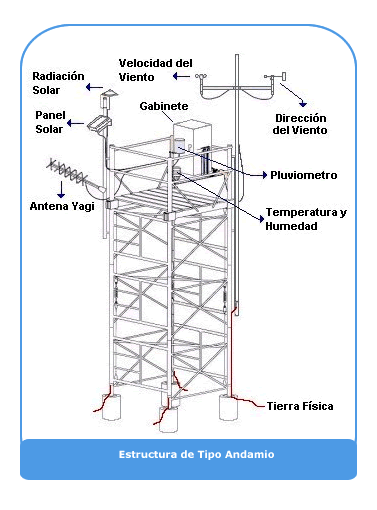
\includegraphics[scale=0.42]{Estacion1.png}
    \label{fig:my_label}
\end{figure}

\subsubsection{Tipo Torre Triangular}

\begin{figure}[h]
    \centering
    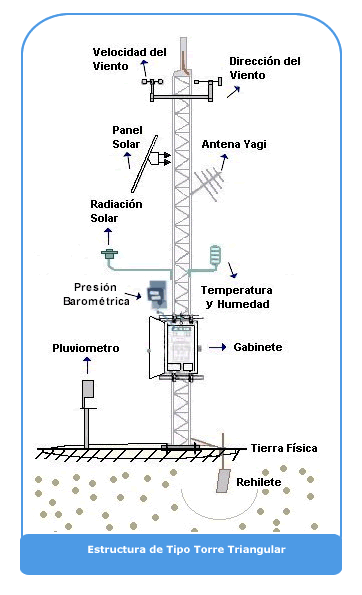
\includegraphics[scale = 0.42]{Estacion2.png}
\end{figure}

\section{Análisis de Datos}

Para comenzar con el análisis fue necesario instalar Python de Anaconda en la versión 3.7. Anaconda incluye Jupyter Lab. Primero creamos una carpeta llamada "Actividad2" para después, desde Anaconda Prompt, abrir Jupyter Lab escribiendo lo mismo estando en la carpeta de la actividad. Una vez abierta la ventana del navegador seleccionamos la opción de Python 3.

Los datos utilizados se descargaron de la página del Servicio Meteorológico Nacional de las Estaciones Automáticas. Se eligió la región de Nogales con los datos registrados desde el 24 hasta el 31 de Enero.

Para empezar a trabajar en python, primero se importaron las bibliotecas Pandas, Numerical Python y Matplot para generar las gráficas.

\begin{center}
    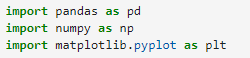
\includegraphics[scale = 1]{Librerias.png}
\end{center}

\noindent Se leyó el archivo de texto, definiéndole una variable, también se saltaron los renglones innecesarios que fueron 4 para después estructurar los datos de mejor manera con \textit{DataFrame}.

\begin{center}
    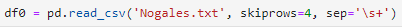
\includegraphics[scale = 1]{read.png}
    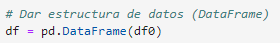
\includegraphics[scale = 1]{DataFrame.png}
\end{center}

A modo de ejemplo se visualizaron los primeros 5 datos obtenidos de la siguiente manera:

\begin{center}
    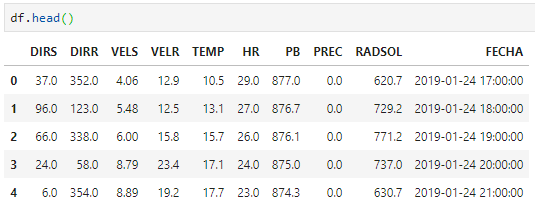
\includegraphics[scale = 1]{head.png}
\end{center}

\section{Resultados}

\noindent Al momento de obtener los resultados, lo que nos interesaba era la variación en el tiempo de la velocidad, ráfagas y su dirección. También se graficó el comportamiento de la radiación solar como función del tiempo. Se realizó una diferencia entre el mínimo y máximo de la temperatura diaria con los datos que arroja el análisis exploratorio de datos.
\clearpage

\subsection{Rapidez del viento, ráfagas y dirección}

Para obtener la rapidez de los vientos y de las ráfagas se usó el siguiente código:
\begin{center}
    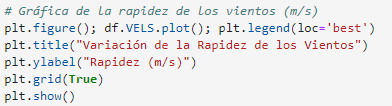
\includegraphics[scale = 1]{Vientos.png}
\end{center}

Sólo se cambió "VELS" por "VELR" para poder graficar la rapidez de las ráfagas:

\begin{center}
    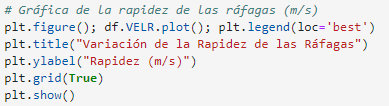
\includegraphics[scale = 1]{Rafagas.png}
\end{center}

\subsubsection{Gráfica de la Rapidez del Viento}

\begin{center}
    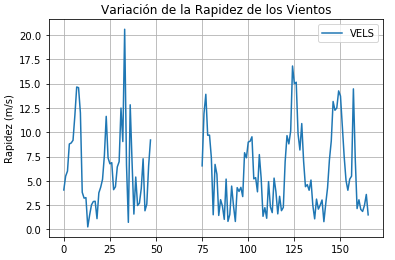
\includegraphics[scale = 1]{GVientos.png}
\end{center}

\subsubsection{Gráfica de la Rapidez de las Ráfagas}

\begin{center}
    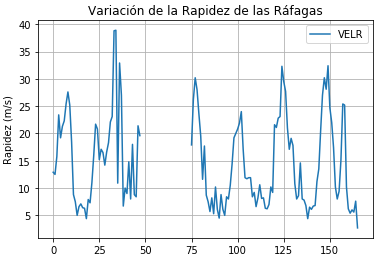
\includegraphics[scale = 1]{GRafagas.png}
\end{center}

Como podemos observar, las horas del día con más viento van desde las 22:00 hasta 03:00 horas.

\subsubsection{Gráfica de la dirección del viento}
Se utilizó el mismo formato del código para generar la gráfica de la variación de la dirección del viento con respecto al viento. 

\begin{center}
    \includegraphics[scale = 1]{Direccion.png}
\end{center}

La gráfica que se generó fue la siguiente
\begin{center}
    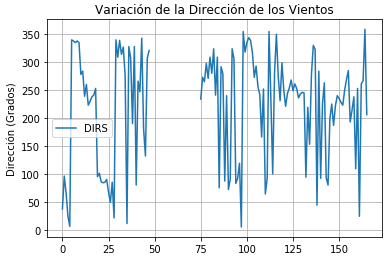
\includegraphics[scale = 1]{GDireccion.png}
\end{center}
Como podemos observar, los vientos dominantes van en la dirección de entre 200 y 300 grados que es en dirección Oeste o Sur-Oeste.

\subsection{Radiación Solar}
El código que se utilizó para generar la gráfica de la radiación solar fue el siguiente:
\begin{center}
    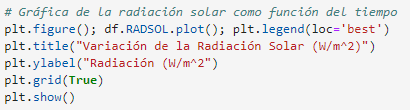
\includegraphics[scale = 1]{Rad.png}
\end{center}
\subsubsection{Gráfica de la Radiación Solar como Función del Tiempo.}

\begin{center}
    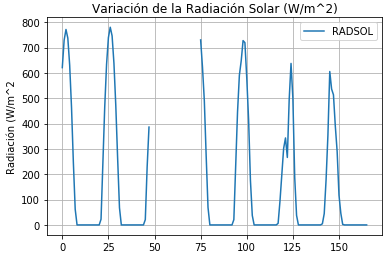
\includegraphics[scale=1]{GRad.png}
\end{center}

La gráfica presenta los valores de la radiación solar en diferentes horas del día, como se puede observar hay un cierto patrón que se forma, aproximadamente las horas con mayor cantidad de radiación son al medio día y por obvias razones se encuentra en 0 en horas de la noche.

\subsection{Temperatura y Humedad}

\subsubsection{Diferencia entre temperatura máxima y mínima}

Para calcular la diferencia se utilizó la función \textit{.min} y \textit{.max} para la columna de las temperaturas y se imprimió la diferencia entre las dos cantidades:
\begin{center}
    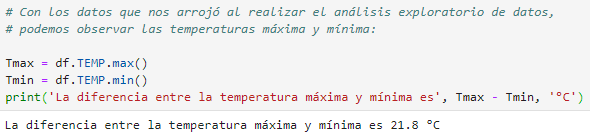
\includegraphics{Temp.png}
\end{center}

\subsubsection{Gráfica de la Humedad Relativa y Temperatura}
\begin{center}
    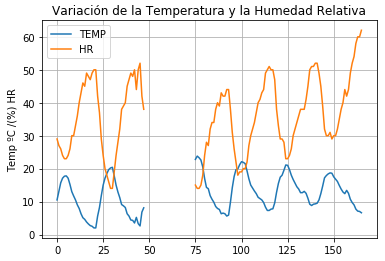
\includegraphics[scale = 1]{GTemp.png}
\end{center}
Como se puede observar en la gráfica, hay una relación entre los dos parámetros. Podemos ver que cuando la temperatura sube, la humedad relativa baja y es lo mismo en sentido contrario.

\subsection{Análisis Exploratorio de Datos}
Para generar el análisis exploratorio sólo fue necesario utilizar la función \textit{describe} sobre nuestro \textit{DataFrame} que nos arrojó una tabla con los siguientes datos.

\begin{center}
    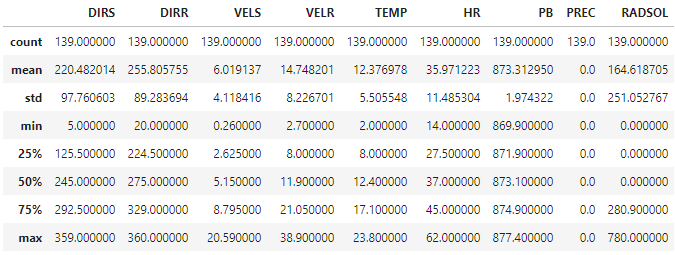
\includegraphics[width = \textwidth]{Describe.png}
\end{center}

\section{Jupyter Lab y Biblioteca Pandas de Python}

\subsection{Jupyter}

Como fue mencionado con anterioridad, Jupyter Notebook es un ambiente de programación que permite editar código, widgets, texto, ecuaciones, imagenes, video, los cuales se pueden convertir a diferentes formatos y compartir facilmente. 
\\

\subsubsection{Características}
Jupyter Notebook contiene tres componentes principales: 
\begin{itemize}
\item Aplicación web: su aplicación interactiva, donde se puede editar y crear código y documentos "notebook". Esta edita y corre código, permite crear widgets de JavaScript e incluye ecuaciones matemática.
\item Kernels: son procesos separados que corren el código del usuario, en cierto lenguaje, en la aplicación web y muestran la salida directamente en la aplicación. Cuenta con kernels que soportan: Phyton, R, Julia, Ruby, Haskell, Scala, node.js, Go.
\item Documentos "notebook": documentos que contienen una representación de lo que se ve en la aplicación web, todas las entradas y salidas, imagenes, ecuaciones, etc. Cada notebook tiene su propio kernel. Los notebooks consisten en una sucesión de celdas y tienen la extensión ".ipynb", pero pueden exportarse en diferentes formatos como PDF o LaTeX.
\end{itemize}

\subsubsection{Ventajas}
\begin{itemize}
\item Se puede usar en prácticamente cualquier lugar, es un software libre disponible en diferentes sistemas operativos y fácil de instalar. 
\item Soporta una amplia variedad de lenguajes de programación, entre los que destaca Phyton, R, Ruby, entre otros.
\item Es interactivo, te brinda inmediatamente el "feedback" o salida del código.
\item Es open source, permite a los usuarios revisarlo y proponer cambios o extensiones, incluso es posible personalizarlo para un uso específico.
\item Produce gráficas, tablas entre otras capacidades matemáticas, es muy utilizado en la ciencia.
\end{itemize}

\subsubsection{Desventajas}
\begin{itemize}
\item Aunque es útil que sea interactivo, es un poco difícil acostumbrarse a esto.
\item Es más complicado instalarlo y acomodarlo todo para un primer uso, que otros entornos de programación. 
\item No es fácil configurarlo para poder compartirlo y editar en otra computadora, es necesario realizar ciertos pasos que no podrían resultar triviales para cualquier usuario.
\item Es difícil poder trabajar de manera colaborativa con este entorno, por lo mismo que no es sencillo "abrir" el código en otra computadora, como se revisó en el punto anterior.
\end{itemize}

\subsection{Phyton: Pandas}

Pandas es un paquete de Phyton que facilita el trabajar con datos. 

Provee estructuras de datos de manera rápida y flexible y promete ser el analista y manipulador de datos, en open source, más poderoso, disponible en cualquier lenguaje. 

Trabaja muy bien en el manejo de varios tipos de datos, ya sean tabulares, datos observacionales o estadísticos, entre otros.

\subsubsection{Ventajas}
\begin{itemize}
\item Reporta cuando se tienen datos perdidos.
\item Permite el cambio de tamaño de los datos, se pueden intertar o eliminar columnas del data frame.
\item Buenas herramientas IO que permiten cargar datos desde archivos planos, bases de datos, archivos excel y guardarlos en un formato HDf5 ultra rápido. 
\item Pandas es rápido.
\item Se usa en la producción de aplicaciones financieras.
\item Permite un manejo de bases de datos bastante extensas.
\item Es fácil de usar y fácil de aprender.
\end{itemize}

\subsubsection{Desventajas}
\begin{itemize}
\item Cuenta con mucha competencia, como es excel, con el que es bastante comparado, ya que también permite el uso de bases de datos, de una manera un poco más sencilla para un usuario no experimentado en el uso de código. 
\end{itemize}


\section{Bibliografía}

\begin{itemize}
    \item Servicio Meteorológico Nacional. (2019). Consultado: 31 de Enero del 2019, de Conagua. Sitio web: http://smn1.conagua.gob.mx/emas/
    \item Python Tutorial (2019). Consultado: 31 de Enero del 2019, de tutorialspoint. Sitio web:
    
    https://www.tutorialspoint.com/python/index.htm
    \item Pros and Cons of Python Jupyter vs Normal Python. (2017). Consultado: 1 de Febrero del 2019, de Quora. Sitio web:
    
    https://www.quora.com/What-are-the-pros-and-cons-of-using-Python-Jupyter-versus-a-normal-Python-development-environment
    
    \item Biblioteca Pandas. (2019). Consultado: 1 de Febrero del 2019, de Pandas Pydata. Sitio web: https://pandas.pydata.org/pandas-docs/stable/index.html
    
\end{itemize}

\section{Apéndice}
\begin{enumerate}
    \item ¿Cuál es tu primera impresión de Jupyter Notebook?
    
    Es muy práctico porque se trabaja todo en una sola carpeta y el código cada cierto tiempo se guarda de manera automática. El manejo de archivos dentro de la misma interfaz es muy cómodo y se pueden abrir desde el mismo \textsc{JupyterLab}.
    
    \item ¿Se te dificultó leer código en Python?
    
    No, de hecho el código que maneja Python es demasiado intuitivo así como las funciones muestran de manera clara su objetivo, es muy práctico y sencillo de aprender. Además no es necesario compilar el código, sólo correrlo.
    
    \item ¿En base a tu experiencia de programación en Fortran, que te parece el entorno de trabajar en Python?
    
    Es mucho más cómo y sencillo, empezando con que no es necesario declarar variables como cierto número entero o de otro tipo. Es más fácil trabajar en el entorno de python que el de Fortran.
    
    \item A diferencia de Fortran, ahora se producen las gráficas utilizando la biblioteca Matplotlib. ¿Cómo fue tu experiencia?.
    
    Primero, es diferente estéticamente a gnuplot de fortran, es muy agradable a la vista y son más fáciles de producir.
    
    \item En general, ¿qué te pareció el entorno de trabajo en Python?
    
    Me pareció muy cómodo, más que nada, en definitiva preferiría seguir programando en Python y dejar otros lenguajes de lado por el momento. Me parece intuitivo, fácil de manejar y de aprender.
    
    \item ¿Qué opinas de la actividad? ¿Estuvo compleja? ¿Mucho material nuevo? ¿Que le faltó o que le sobró? ¿Qué modificarías para mejorar?
    
    Sólo fue un poco laboriosa al momento de escribir el reporte en \LaTeX, pero sólo es por falta de práctica. En general, la actividad es sencilla, sí hay material nuevo porque no conocía bien el entorno de python y menos el de JupyterLab. 
    
    \item ¿Comentarios adicionales que desees compartir?
    
    Ya había entrado a programar en python desde el semestre pasado para la materia de "Análisis Numérico" donde se me pidió calcular numéricamente las constantes elásticas y otras cosas en el problema de oscilador armónico. Me gustaría seguir aprendiendo python en otras áreas para encontrar más aplicaciones, en especial la inteligencia artificial junto con el análisis de datos. 
\end{enumerate}



 
 
 











\end{document}


